\chapter{Irradiation Tests}
\label{chap:II-6-irradiation}

  The OptoHybrid will be located in a region of CMS exposed to high fluxes of particles, some of which might interact with the FPGA and generate errors in the logic. Those could in turn influence the functioning of the system and degrade its performance. To solve this issue, irradiation tests have been performed to measure the interaction cross-section of the particles with the various components of the FPGA. Two OptoHybrids have been placed in a high intensity proton beam with a dedicated firmware designed to detect errors. The two boards were each controlled by an additional OptoHybrid placed outside the test area which recorded the events and statistics. \\

  In this chapter, we provide the user with an overview of the internal architecture of an FPGA to better understand the potential sources of errors. We then describe the firmware of the irradiated and control FPGAs which has been used during the test. The setup and beam parameters of the irradiation test are reviewed before presenting the results that were obtained after analysis.

  \section{Architecture of an FPGA}

    To optimize the occupancy of the resources of the FPGA and develop code that uses the full potential of the device, a deep comprehension of the intrinsic architecture of the chip is required. To this end, a description of the building blocks of the FPGA is given.

    \subsection{Configurable Logic Blocks}

      (CLBs) \cite{VIRTEX-CLB} are the base elements of the FPGA used to implement sequential and combinatorial logic. They are composed of two important objects: look-up tables (LUTs) and registers. LUTs are components which outputs are a function of the inputs as defined in a programmable table. They implement a truth table for every possible combination of the inputs which defines the value of the outputs. The response of a LUT to a change in the inputs is almost instantaneous. LUTs in the Xilinx Virtex-6 FPGAs can either implement functions with six inputs and a single output or functions with five inputs and two outputs. The outputs of the LUTs can, if so required by the design, be connect to registers which sample the signals at the rising edge of a given clock. Register are used for their sample-and-hold functionality which makes designs synchronous to clocks. With these two components, CLBs can implement complex functions and describe intricate systems. \\

      Each CLB is composed of two slices each made of four LUTs and eight register which layout is shown in Figure \ref{fig:II-6-clb}. Each LUT is connected to an input bus of six signals (A, B, C, and D inputs) and to an unbuffered output bus of a single bit (O6 to A, B, C, and D). Four additional signals enter the slice (AX, BX, CX, and DX) and are connected to multiplexers (red) which allows to buffer either the former or the second output of the LUTs (O5). The output of the same buffer is then connected to a second multiplexer (orange) which allows to select either the former or an unbuffered output of the LUTs (AMUX, BMUX, CMUX, and DMUX). Finally, a third multiplexer (green) connects a range of signals to the registers on the right which are then connected to four outputs (AQ, BQ, CQ, and DQ). Three additional multiplexers (blue) offer the possibility to mix the signals from the four LUTs to generate a wider range of logical operations. The flexibility offered by this architecture is what enables FPGAs to implement complex designs. The Xilinx Virtex-6 FPGA used in the OptoHybrid v2a (XC6VLX130T) holds 10 000 CLBs with a total of 80 000 LUTs and 160 000 registers.

      \begin{figure}[p!]
        \centering
        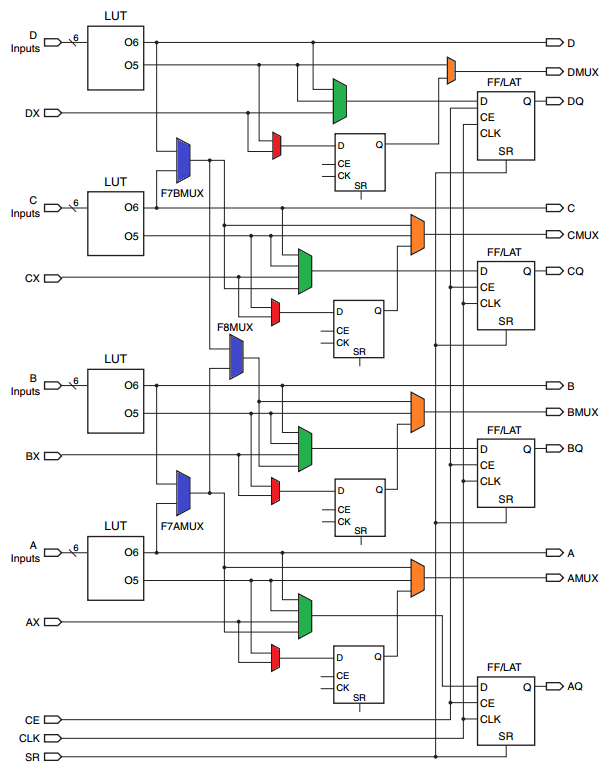
\includegraphics[width=\textwidth]{img/II-6-irradiation/clb.png}
        \caption{Simplified view of a slice composed of four LUTs on the left and eight registers on the right \cite{VIRTEX-CLB}.}
        \label{fig:II-6-clb}
      \end{figure}

    \subsection{The switching matrix}

      is what connects CLBs with each other. It is a vast network of switches which are used to route signals between components. The open/closed status of each switch is programmable and defines the routes signals take inside the vast network of connections.

    \subsection{Block RAM}

      are dedicated storage elements present inside the FPGA which are not programmable in advance but are used to store data during run. Block RAMs can store up to 36 kb of data which can be configured in different ways: 32K x 1 bit, 16K x 2 bits, etc. They can also be used as first in first out (FIFO) modules which are similar to data queues.

    \subsection{Digital Signal Processing}

      units or DSPs are modules which perform additions, subtractions, and multiplications using dedicated hardware elements. They are used to quickly solve mathematical problems without relying on CLBs which can consume large amount of resources to perform an equivalent task.

    \subsection{The configuration memory}

      is what makes an FPGA flexible: it holds the configuration of every single LUT, switching matrix element, etc. It defines the truth table of LUT, parametrizes the DSP, defines the connection between elements, etc. It is what implements the design in the FPGA. By nature, the configuration memory is volatile and will lose its configuration upon power down or reset. To reload it, the FPGA tries to read it out of an attached memory device or remains in a blank state if it fails to do so.

  \section{Firmware Design for the Irradiated FPGA}

    The firmware of the irradiated FPGA is design to use a maximum of the available resources and transmit any error detected during run time.

    \subsection{Configurable Logic Block}

    \subsection{Block RAM}

    \subsection{Digital Signal Processing}

    \subsection{Soft Error Mitigation}

  \section{Firmware Design for the Control FPGA}

    \subsection{Communication Protocol}

    \subsection{ChipScope Core}

  \section{Irradiation Setup}

  \section{Data Analysis}

  \section{Conclusion}
